
\section{Results}
\label{outflows:sec:results}

\subsection{Radial Gradients}
\label{outflows:sec:empirical:gradients}

Fig.~\ref{outflows:fig:age-xh-dists} shows age and abundance distributions of
our sample in bins of Galactocentric radius.
Stars tend to be young in the outer Galaxy, where the age distributions have a
peak around~$\sim$$2-4$ Gyr and a tail toward older ages.
As radius increases, the age distribution shifts to a peak at older ages and a
skew-negative tail.
This result is a natural consequence of inside-out Galaxy formation, whereby
the inner regions of the disk assemble at high redshift and the outer regions
follow suit on longer timescales~\citep[e.g.,][]{White1991, Bird2013}.
Abundances follow a similar pattern, shifting from a metal-rich mode and
skew-negative tail to a metal-poor mode and skew-positive tail with increasing
radius (a result previously found in APOGEE by~\citealt{Hayden2015}).
These bulk shifts in stellar population properties with radius are indicative
of radial gradients, which we quantify in more detail below.

% \afterpage{
% \clearpage
\begin{landscape}
\begin{figure*}
\centering
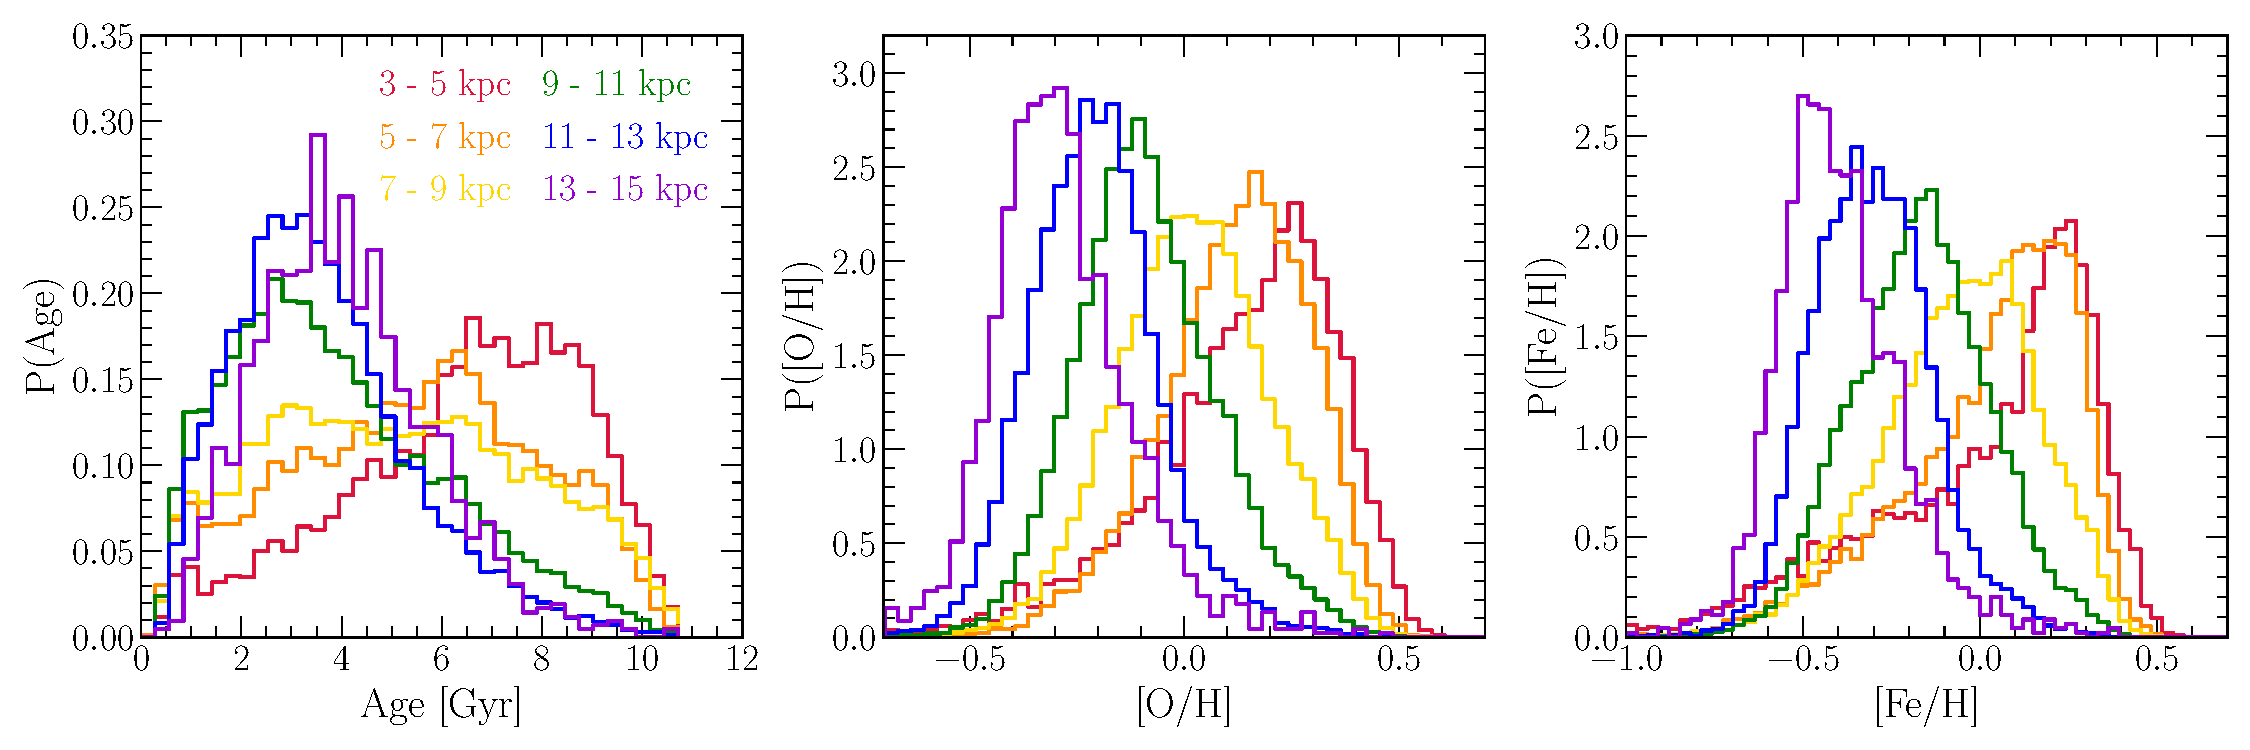
\includegraphics[scale = 0.55]{age_xh_dists.pdf}
\caption{
Age (left) and abundance (middle and right) distributions from our APOGEE
sample (see discussion in~\S~\ref{outflows:sec:empirical:apogee}) at different
radii.
Within each 2-kpc wide bin in radius, we box-car smooth the distribution with a
width of~$\Delta \tau = 1$ Gyr in age and~$\Delta$[X/H] = 0.2 for both O and
Fe.
}
\label{outflows:fig:age-xh-dists}
\end{figure*}
\end{landscape}
% \clearpage
% }

To quantify the gradients in our sample, we first sort stars into 1-kpc wide
bins in Galactocentric radius.
We then compute the median age~$\tau_{1/2}$ and the 16th and 84th percentiles
of the distribution by simply sorting the values into ascending order.
The left panel of Fig.~\ref{outflows:fig:gradxh-gradage} shows the results of
this procedure.
Our sample is large enough that bootstrap error estimates indicate statistical
uncertainties smaller than the points in the figure.
A linear regression indicates a median trend of~$\gradage = -0.375 \pm 0.036$
Gyr/kpc with an intercept of~$8.21 \pm 0.31$ Gyr.
The median age closely follows this line of best fit at~$R \lesssim 9$ kpc, but
flattens off in the outer disk and reverses sign slightly.

\begin{figure*}
\centering
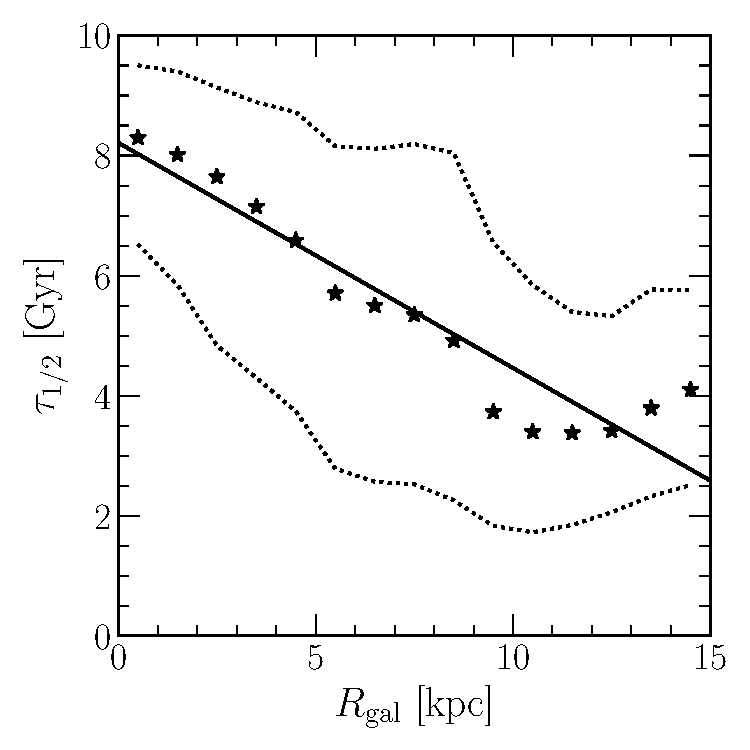
\includegraphics[scale = 0.51]{age_gradient.pdf}
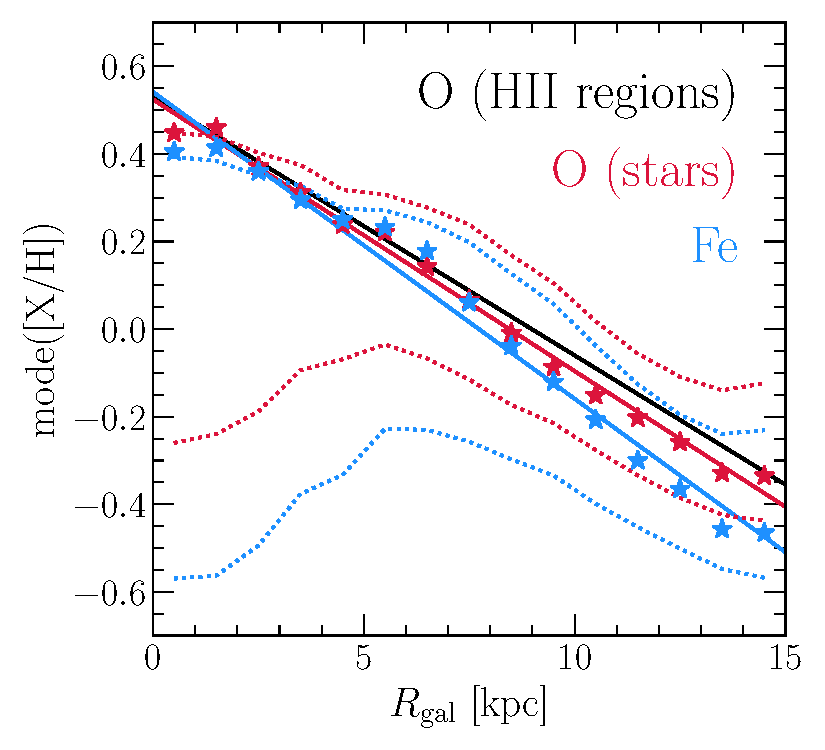
\includegraphics[scale = 0.5]{gradxh.pdf}
\caption{
Gradients in stellar age (left) and metallicity (right; red for O and blue for
Fe).
Stars denote the median age and mode abundance in 1-kpc bins of radius, with
dotted lines marking the 16th and 84th percentiles of the distributions in each
radial bin.
Solid lines denote the lines of best fit applied to the corresponding summary
statistics, with the fit parameters summaries in Table X.
The black line in the right hand panel marks the O abundance gradient in
Galactic HII regions measured by~\citet{MendezDelgado2022}.
}
\label{outflows:fig:gradxh-gradage}
\end{figure*}

Though we quantify the age gradient in terms of the median trend, the mode is
our summary statistic of choice in quantifying metallicity gradients.
We discuss our motivation behind this choice in~\S~{\color{red} X}.
In short, our GCE models suggest that the mode is not significantly affected
by stellar migration, {\color{red} except perhaps in the outermost regions of
the disk(?).}
Consequently, its variations should reflect the enrichment histories of
different Galactic regions with little contamination.
Because the mode is a noisy statistic, we fit a skewed normal distribution to
the MDF in each radial bin and determine the mode by optimization.
We however estimate the 16th and 84th percentiles by simply sorting the
abundances into ascending order as we did for the age distributions.
\par
The right panel of Fig.~\ref{outflows:fig:gradxh-gradage} shows the resultant
gradients in~\oh~and~\feh\footnote{
	We follow conventional notation where
	[X/Y]~$\equiv \log_{10} (N_x / N_y) - \log_{10} (N_x / N_y)_\odot$
}.
As expected given the MDFs in Fig.~\ref{outflows:fig:age-xh-dists}, stars tend
to decline in metallicity with increasing radius.
Linear regressions indicate slopes of~$\grad{O} = -0.062 \pm 0.001$ kpc$^{-1}$
and~$\grad{Fe} = -0.070 \pm 0.003$ kpc$^{-1}$, in reasonable agreement with
previous measurements (see discussion in~\S~\ref{outflows:sec:intro} and
references therein).
Our GCE models {\color{red} successfully(?)} reproduce the slightly steeper
slope in Fe; we describe the origin of this result in~\S~{\color{red} X}.
For comparison, we additionally plot~\citeauthor{MendezDelgado2022}'s
\citeyearpar{MendezDelgado2022} fit to the gas-phase O gradient traced by
Galactic HII regions accounting for their temperature inhomogeneities.
The two O gradients are consistent within their~$1\sigma$ uncertainties.
% \par
% We use these measurements to calibrate our GCE models
% in~\S~\ref{outflows:sec:gce} below.
% We quantify the abundance gradients conditioned on stellar age and compare
% against our models in~\S~\ref{outflows:sec:results}.

\subsection{Evolution of the Abundance Gradient}
\label{outflows:sec:empirical:evolution}

\begin{figure*}
\centering
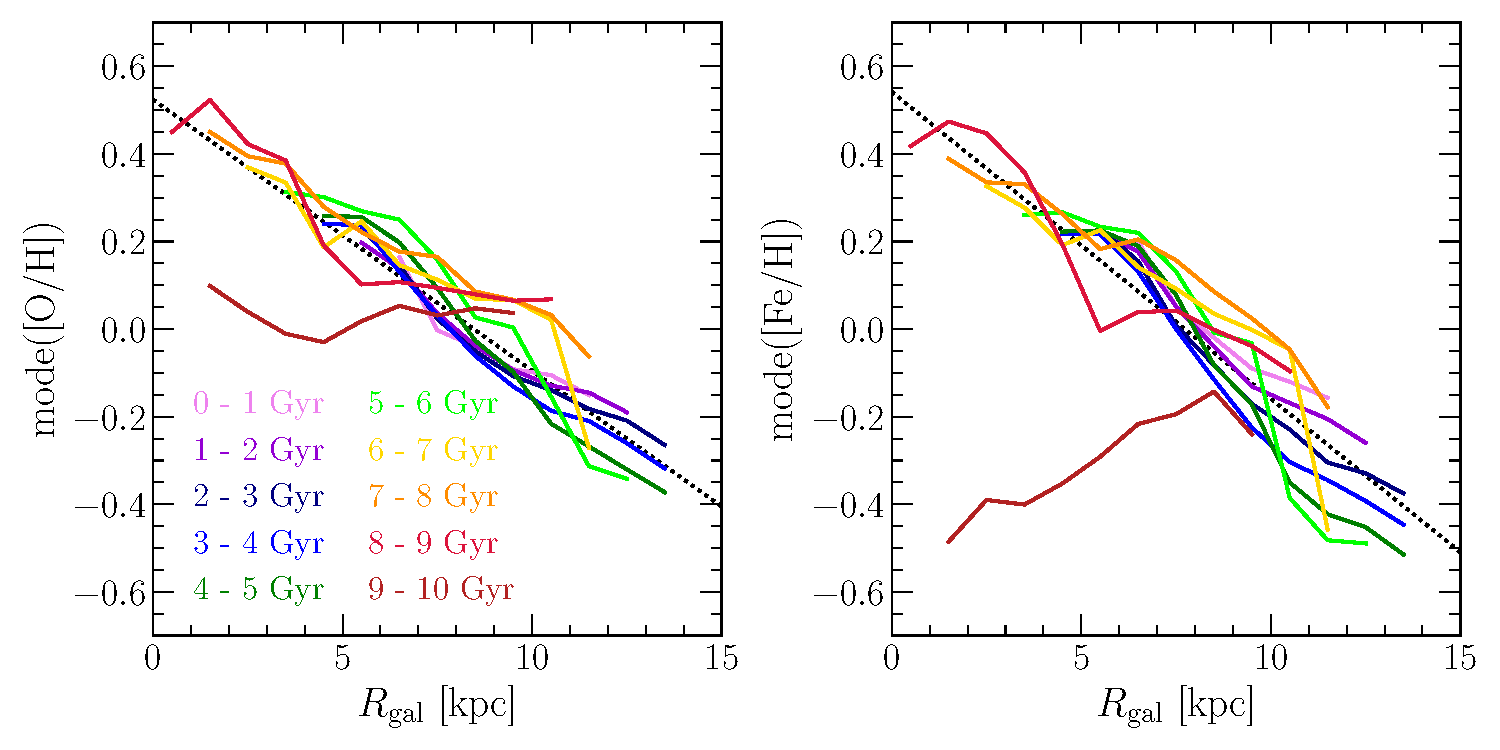
\includegraphics[scale = 0.55]{gradxh_fixedage.pdf}
\caption{
Radial gradients in [O/H] (left) and [Fe/H] (right) conditioned on stellar age
in 1-Gyr bins according to the legend in the left panel.
}
\label{outflows:fig:gradxh-fixed-age}
\end{figure*}


{
\renewcommand{\arraystretch}{1.3}
\begin{table*}
\caption{
A summary of our linear regressions in age and metallicity gradients (see
discussion in~\S~\ref{outflows:sec:empirical:gradients}).
}
\begin{tabularx}{\columnwidth}{c @{\extracolsep{\fill}} l l l}
\toprule
Subsample & Slope & Intercept & $\chi_\text{dof}^2$
\\
\toprule
\multicolumn{4}{c}{\textbf{Age}}
\\
All Stars & $-0.375 \pm 0.036$ Gyr kpc$^{-1}$ & $8.21 \pm 0.31$ Gyr & --
\\
\midrule
\multicolumn{4}{c}{\textbf{\oh}}
\\
All Stars & $-0.062 \pm 0.001$ kpc$^{-1}$ & $0.524 \pm 0.013$ & $0.004$
\\
$0 - 1$ Gyr & $-0.055 \pm 0.011$ kpc$^{-1}$ & $0.459 \pm 0.103$ & $0.146$
\\
$1 - 2$ Gyr & $-0.056 \pm 0.005$ kpc$^{-1}$ & $0.473 \pm 0.048$ & $0.082$
\\
$2 - 3$ Gyr & $-0.059 \pm 0.005$ kpc$^{-1}$ & $0.497 \pm 0.052$ & $0.129$
\\
$3 - 4$ Gyr & $-0.066 \pm 0.004$ kpc$^{-1}$ & $0.544 \pm 0.038$ & $0.169$
\\
$4 - 5$ Gyr & $-0.079 \pm 0.004$ kpc$^{-1}$ & $0.662 \pm 0.037$ & $0.055$
\\
$5 - 6$ Gyr & $-0.080 \pm 0.007$ kpc$^{-1}$ & $0.690 \pm 0.062$ & $0.093$
\\
$6 - 7$ Gyr & $-0.055 \pm 0.008$ kpc$^{-1}$ & $0.515 \pm 0.062$ & $0.225$
\\
$7 - 8$ Gyr & $-0.049 \pm 0.002$ kpc$^{-1}$ & $0.517 \pm 0.015$ & $0.320$
\\
$8 - 9$ Gyr & $-0.049 \pm 0.007$ kpc$^{-1}$ & $0.498 \pm 0.047$ & $0.251$
\\
$9 - 10$ Gyr & $-0.001 \pm 0.005$ kpc$^{-1}$ & $0.037 \pm 0.031$ & $0.279$
\\
\midrule
\multicolumn{4}{c}{\textbf{\feh}}
\\
All Stars & $-0.070 \pm 0.003$ kpc$^{-1}$ & $0.541 \pm 0.026$ & $0.023$
\\
$0 - 1$ Gyr & $-0.068 \pm 0.010$ kpc$^{-1}$ & $0.587 \pm 0.091$ & $0.083$
\\
$1 - 2$ Gyr & $-0.072 \pm 0.005$ kpc$^{-1}$ & $0.603 \pm 0.051$ & $0.040$
\\
$2 - 3$ Gyr & $-0.077 \pm 0.006$ kpc$^{-1}$ & $0.613 \pm 0.056$ & $0.020$
\\
$3 - 4$ Gyr & $-0.083 \pm 0.005$ kpc$^{-1}$ & $0.617 \pm 0.048$ & $0.039$
\\
$4 - 5$ Gyr & $-0.096 \pm 0.007$ kpc$^{-1}$ & $0.735 \pm 0.062$ & $0.090$
\\
$5 - 6$ Gyr & $-0.097 \pm 0.012$ kpc$^{-1}$ & $0.746 \pm 0.104$ & $0.205$
\\
$6 - 7$ Gyr & $-0.066 \pm 0.012$ kpc$^{-1}$ & $0.541 \pm 0.089$ & $0.102$
\\
$7 - 8$ Gyr & $-0.051 \pm 0.004$ kpc$^{-1}$ & $0.493 \pm 0.028$ & $0.185$
\\
$8 - 9$ Gyr & $-0.061 \pm 0.008$ kpc$^{-1}$ & $0.504 \pm 0.049$ & $0.048$
\\
$9 - 10$ Gyr & $0.038 \pm 0.006$ kpc$^{-1}$ & $-0.510 \pm 0.037$ & $0.380$
\\
\bottomrule
\end{tabularx}
\label{outflows:tab:apogee-regressions}
\end{table*}
}


\begin{figure}
\centering
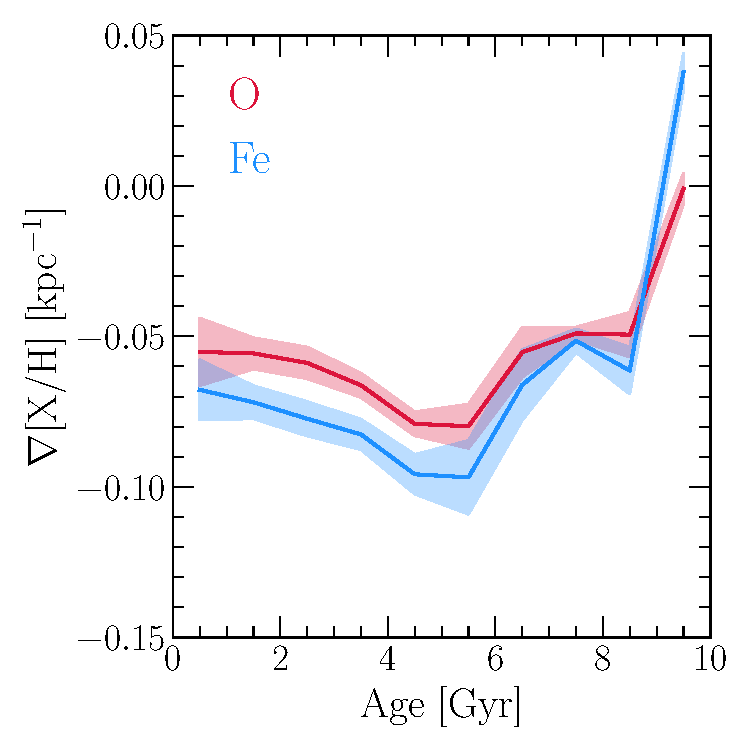
\includegraphics[scale = 0.6]{gradxh_vs_age.pdf}
\caption{
The slope of the radial abundance gradient in O (red) and Fe (blue) in 1-Gyr
bins of stellar age (see discussion
in~\S~\ref{outflows:sec:empirical:gradients}).
}
\label{outflows:fig:gradxh-vs-age}
\end{figure}

As a central interest of this chapter is to quantify the evolution of the
Galactic abundance gradient over time, we now repeat these measurements
conditioned on stellar age.
In conditioning on both age and radius, we fit for the mode of the MDF only in
bins containing at least 200 stars.
This is a sufficiently large sample in each bin such that bootstrap resampling
indicates statistial uncertainties in the mode comparable to the width of the
lines plotted ($\lesssim0.1\%$).
\par
Fig.~\ref{outflows:fig:gradxh-fixed-age} shows the gradients themselves in each
age bin.
We also report slopes and intercepts from linear regressions to the trend in
each age bin in Table~\ref{outflows:tab:apogee-regression} and visualize the
inferred gradients in Fig.~\ref{outflows:fig:gradxh-vs-age}.
To first order, the gradient was established~$\sim$$8 - 9$ Gyr ago.
In the oldest age bin, the abundance profile is consistent with flat in~\oh~but
is positively sloped in~\feh.
The gradient held relatively steady at~$\grad{O} \approx \grad{Fe} \approx
-0.05$ kpc$^{-1}$ for~$\sim$3 Gyr, then steepened to~$\grad{O} \approx -0.07$
kpc$^{-1}$ and~$\grad{Fe} \approx -0.09$ kpc$^{-1}$ before gradually returning
to~$\grad{O} \approx \grad{Fe} \approx -0.05$ kpc$^{-1}$ until the present day.
Inspection of fig.~\ref{outflows:fig:gradxh-fixed-age} indicates that the
steepening of the gradient coincides with a decrease in metallicity
of~$\sim$$0.2 - 0.3$ dex in O and~$\sim$$0.4 - 0.5$ dex in Fe
at~$R_\text{gal} \gtrsim$8 kpc.
\par
{\color{red} Potentially move to discussion section.}
This result is readily explained by a dilution event due to accretion of
metal-poor gas in the outer disk.
A decrease in metallicity indicates that the enrichment rate and by extension
the SFR are slow relative to the infall rate.
A burst in star formation driven by the increased resources then naturally
ensues~\citep[e.g.,][]{Dalcanton2007}.
The differences in both the magnitude of the dilution in
Fig.~\ref{outflows:fig:gradxh-fixed-age} and the timescales in
Fig.~\ref{outflows:fig:gradxh-vs-age} between O and Fe are expected under this
scenario.
[O/H] and [Fe/H] decrease by the same amount only the limit that the
accretion event is instantaneous~\citep{Johnson2020}, and O re-enrichment is
faster due to the restitution delay of SN Ia Fe yields.

\subsection{Caveats}
\label{outflows:sec:empirical:caveats}
Since our sample was produced by training~\textsc{AstroNN}'s deep learning
capabilities on APOGEE spectra, our ages may be biased by known correlations
with abundances (e.g., the age-[O/Fe] relation,~\citealt{Feuillet2019}).
To assess the impact of this decision, we have remade our measurements
in~\S\S~\ref{outflows:sec:empirical:apogee} and~\ref{outflows:sec:results}
with the~\citet{Leung2023} age catalog.
They mitigate this potential issue by compressing the spectra into lower
dimensional representations of themselves (i.e., a~\textit{latent space}) using
a variational encoder-decoder algorithm~\citep[e.g.,][]{LeCun2015}.
They then train a modified random forest algorithm to predict similarly
compressed lightcurves trained on~\textit{Kepler} photometry
\citep{Borucki2010}.
They demonstrate that this latent space contains little if any information on
chemical abundances and stellar parameters, as intended, after which they are
able to estimate ages by augmenting the latent space with~$T_\text{eff}$
and~$\log g$ and decompressing the lightcurves.
\par
We find similar results with either age catalog, indicating that any biases
introduced by abundance information in the APOGEE spectra is of little to no
concern.
Though the value added catalog exhibits a dearth of very old stars
($\gtrsim$$10$ Gyr; see Fig.~\ref{outflows:fig:age-xh-dists} and Fig. 11 of
\citealt{Leung2023}), this should not be a problem for this chapter since we
are primarily interested in~$\lesssim$$10$ Gyr old populations anyway.
The main advantage of the value added catalog over~\citet{Leung2023} is that
their ages are available only for stars with surface gravities
of~$\log g = 2.5 - 3.6$ due to their training sample.
As a result, the value added catalog is a factor of~$\sim$$2.5$ large, yielding
much more precise summary statistics.
This decision also provides better coverage of the Galactic disk as we are able
to use luminous, low-surface gravity stars on the upper red giant branch.
\par
Particularly with regard to our measurement of the age gradient, the APOGEE
selection function is a significant source of systematic uncertainty.
APOGEE primarily targets stars with 2MASS~\citep{Skrutskie2006} magnitudes
of~$7 < H < 13.8$ on a grid of sightlines at Galactic latitudes
$b = 0$,~$\pm 4^\circ$, and~$\pm 8^\circ$ (targeting is described in detail
by~\citealt{Zasowski2013, Zasowski2017, Beaton2021}, and~\citealt{Santana2021}).
Quantifying the impact of this sampling bias in APOGEE first requires relating
a star's apparent magnitude and color to a selection fraction based on its
location on the 2-D sky~\citep{Bovy2016c, Mackereth2017, Lian2022}.
One must then combine this mapping with a 3-D dust map to account for reddening
and some model of the intrinsic number density of potential targets based on
stellar properties from isochrones and an initial mass function (IMF; e.g.
\citealt{Kroupa2001, Chabrier2003}), which then results in the selection
fraction as a function of Galactic position, metallicity, and age
\citep[see also][]{Mackereth2020}.


% \subsection{Simplified Examples}
% \label{outflows:sec:simplified-example}

% We begin by comparing the fiducial model from Chapter~\ref{migration} with a
% simplified model in which~$\eta = 0$ to highlight generic differences between
% models with and without mass loading.
% In Chapter~\ref{migration}, the strength of mass loading increases
% exponentially with radius according to
% \begin{equation}
% \eta = \frac{\ycc{O}}{Z_{\text{O},\odot}}
% e^{-\grad{O} (\ln 10) (R - R_\odot)} + r - 1.
% \end{equation}
% Under this parameterization, the equilibrium abundance~$Z_\text{O}$ scales with
% radius according to the specified gradient~\grad{O}.
% In the case of~$\eta = 0$, the stellar gradient instead arises out of a handful
% of effects, including less efficient star formation (i.e., higher~$\tau_\star$)
% and a more extended SFH (i.e., high~$\timescale{sfh}$) with increasing radius.
% \par
% We calibrate a model with~$\eta = 0$ everywhere such that the mode of the MDF
% scales with radius according to the gradient we measured
% in~\S~\ref{outflows:sec:empirical:gradients}.
% The distribution in~$Z$ for some element can be expressed as
% \begin{equation}
% \frac{dN}{d \ln Z} = Z \frac{dN / dt}{dZ / dt}
% \propto \frac{\dot{M}_\star}{(\dot{Z} / Z)}.
% \end{equation}
% By differentiating the above expression and making a handful of additional
% chain rule substitutions, it is straightforward to show that
% \begin{equation}
% \frac{d^2N}{d \ln Z^2} \propto \dot{M}_\star
% \left(\frac{Z}{\dot{Z}}\right)^2
% \left(
% \frac{\ddot{M}_\star}{\dot{M}_\star} + \frac{\dot{Z}}{Z} -
% \frac{\ddot{Z}}{\dot{Z}}
% \right).
% \end{equation}
% Herein lies a portion of our motivation for choosing the mode as our summary
% statistic in quantifying abundance gradients.
% From the above expression, it is clear that the peak of the MDF is produced
% when
% \begin{equation}
% \frac{\ddot{M}_\star}{\dot{M}_\star} = \frac{\ddot{Z}}{\dot{Z}} -
% \frac{\dot{Z}}{Z},
% \end{equation}
% allowing one to solve for the time at which the peak is produced to determine
% its position.
% For simple SFHs, such as those in~\S~\ref{outflows:sec:gce:onezone:simple-cases},
% the solution is straightforward since one can express~$Z_\text{O}(t)$
% analytically.
% \par
% In the case of a single exponential SFH, differentiating
% $\dot{M}_\star \propto e^{-t / \tau_\text{sfh}}$ and
% $f_\text{sfh} = 1 - e^{-t / \taupsi{O}}$ (see
% Table~\ref{outflows:tab:f-sfh-forms}) and solving for the time~$t_\text{max}$
% at which the turnover in the MDF is produced yields
% \begin{equation}
% t_\text{max} = -\taupsi{O} \ln \left(1 - \frac{\timescale{sfh}}{\taupsi{O}}
% \right).
% \end{equation}
% Computing~\oh~based on~$f_\text{sfh}(t_\text{max})$ indicates that the mode
% occurs at
% \begin{equation}
% \text{mode([O/H])} = \log_{10}
% \left(\frac{\ycc{O} \timescale{sfh}}{Z_{\text{O},\odot} \tau_\star}\right).
% \end{equation}
% \par
% In principle, the mode will shift due to changes in both~$\tau_\star$ and
% \timescale{sfh}.
% Since this is a deliberately simplified example, we do not use the three
% component power-law~$\dot{\Sigma}_\star - \Sigma_g$ relationship as in the
% $\eta > 0$ comparison case (see discussion below).
% We instead take a single power-law, enabling a straightforward solution
% for~$\tau_\star$ and therefore~\timescale{sfh} as a function of radius.
% By definition,
% \begin{equation}
% \begin{split}
% \Sigma_g \tau_\star^{-1} &\propto \Sigma_g^N
% \\
% \tau_\star & \propto \Sigma_g^{1 - N}
% \\
% & \propto e^{(N - 1) R / R_g},
% \end{split}
% \end{equation}
% where~$N$ is the power-law index of the~$\dot{\Sigma}_\star - \Sigma_g$
% relation and~$R_g$ is the scale radius of the gas disk.
% Combining terms, solving for~$\timescale{sfh}$, and replacing mode([O/H]) with
% the desired abundance gradient yields the following relationship between
% \timescale{sfh} and~$R$:
% \begin{equation}
% \tau_\text{sfh} = \tau_{\star,0} \frac{Z_{\text{O},\odot}}{\ycc{O}}
% \exp\left[
% (N - 1)\frac{R}{R_g} + \grad{O}(\ln 10)(R - R_\odot)
% \right],
% \label{outflows:eq:tausfh-simplified}
% \end{equation}
% where~$\tau_{\star,0}$ simply sets the value of~$\tau_\star$ at~$R = 0$,
% $Z_{\text{O},\odot}$ is the O abundance in the Sun, and~$R_\odot = 8$ kpc is
% the Galactocentric radius of the Sun.
% We take~$\grad{O} = -0.06$ kpc$^{-1}$ from our measurements
% in~\S~\ref{outflows:sec:empirical:gradients}.
% We adopt~$N = 1.5$ based on the global SFRs and surface densities of
% low-redshift star forming spirals~\citep{Kennicutt1998}.
% Based on the presence of the central molecular zone in the inner few hundred
% pc of the Galaxy~\citep[e.g.,][]{Morris1996, Dahmen1998, PiercePrice2000,
% Hatchfield2020} and~\citeauthor{Leroy2008}'s~\citeyearpar{Leroy2008}
% measurement of~$\tau_\star \approx 2$ Gyr for purely molecular gas, we
% attribute this value to~$\tau_{\star,0}$.
% We take a scale radius of the gas disk~$R_g = 3$ kpc so that~\timescale{sfh}
% increases with radius, as expected from inside-out Galaxy growth
% (equation~\ref{outflows:eq:tausfh-simplified} suggests there is a region of
% parameter space at high~$R_g$ where the timescale decreases with radius).

% \begin{figure*}
% \centering
% 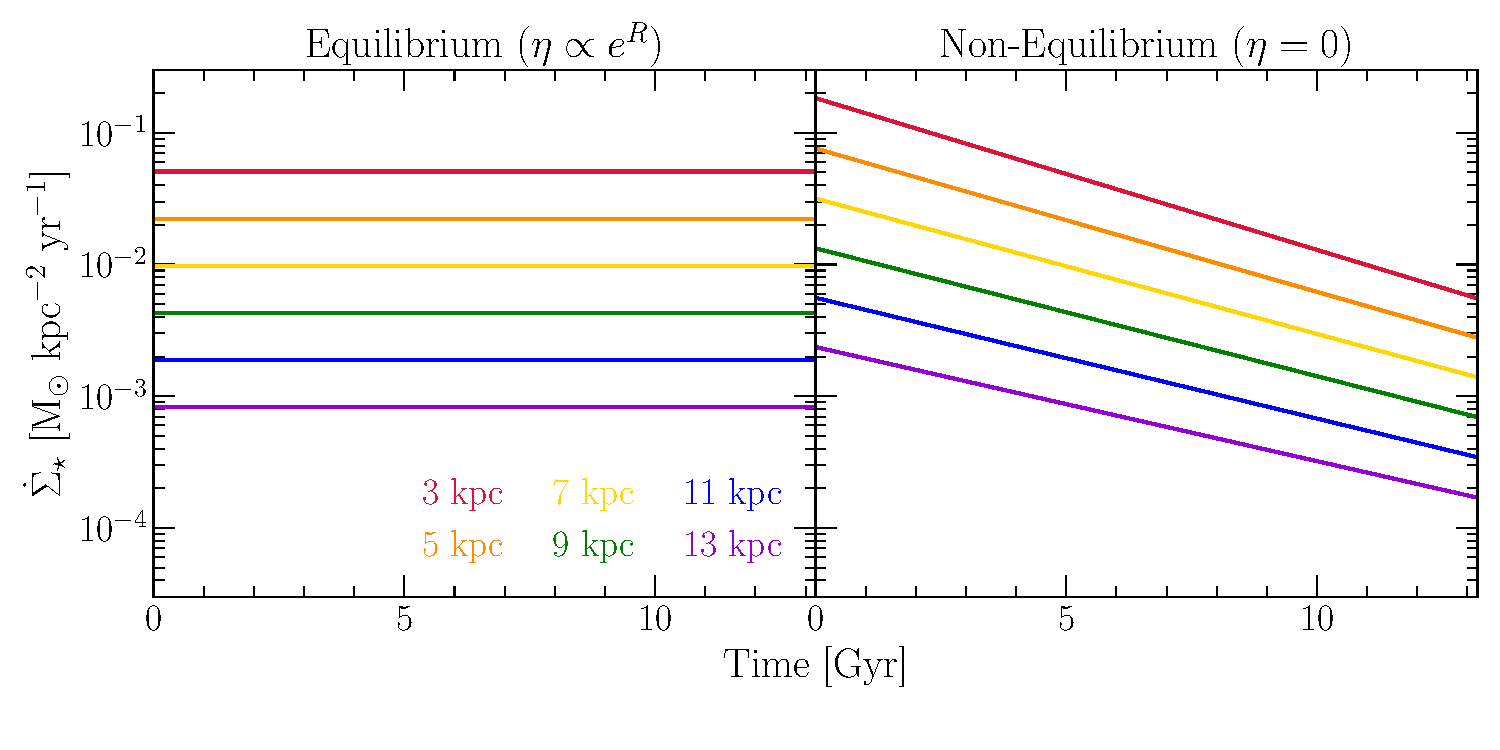
\includegraphics[scale = 0.5]{simplified-examples-sfhs.pdf}
% \caption{
% SFHs of the~$\eta \propto e^R$ (left) and the~$\eta = 0$ (right) simplified
% examples.
% Each curve shows the time dependence at a specific radius, color coded
% according to the legend.
% }
% \label{outflows:fig:simplified-examples-sfhs}
% \end{figure*}

% For a comparison case with~$\eta \neq 0$, we take the model from
% Chapter~\ref{migration} with a constant SFH.
% In this scenario, it is not the SFH that must be calibrated to the abundance
% gradient but~$\eta$ as a function of~$R$.
% In Chapter~\ref{migration}, we took an exponential scaling
% \begin{equation}
% \eta = \frac{\ycc{O}}{Z_{\text{O},\odot}}
% e^{-\grad{O}(R - R_\odot)} + r - 1,
% \end{equation}
% such that the equilibrium abundance varied with radius according to empirical
% gradient.

% \begin{figure*}
% \centering
% 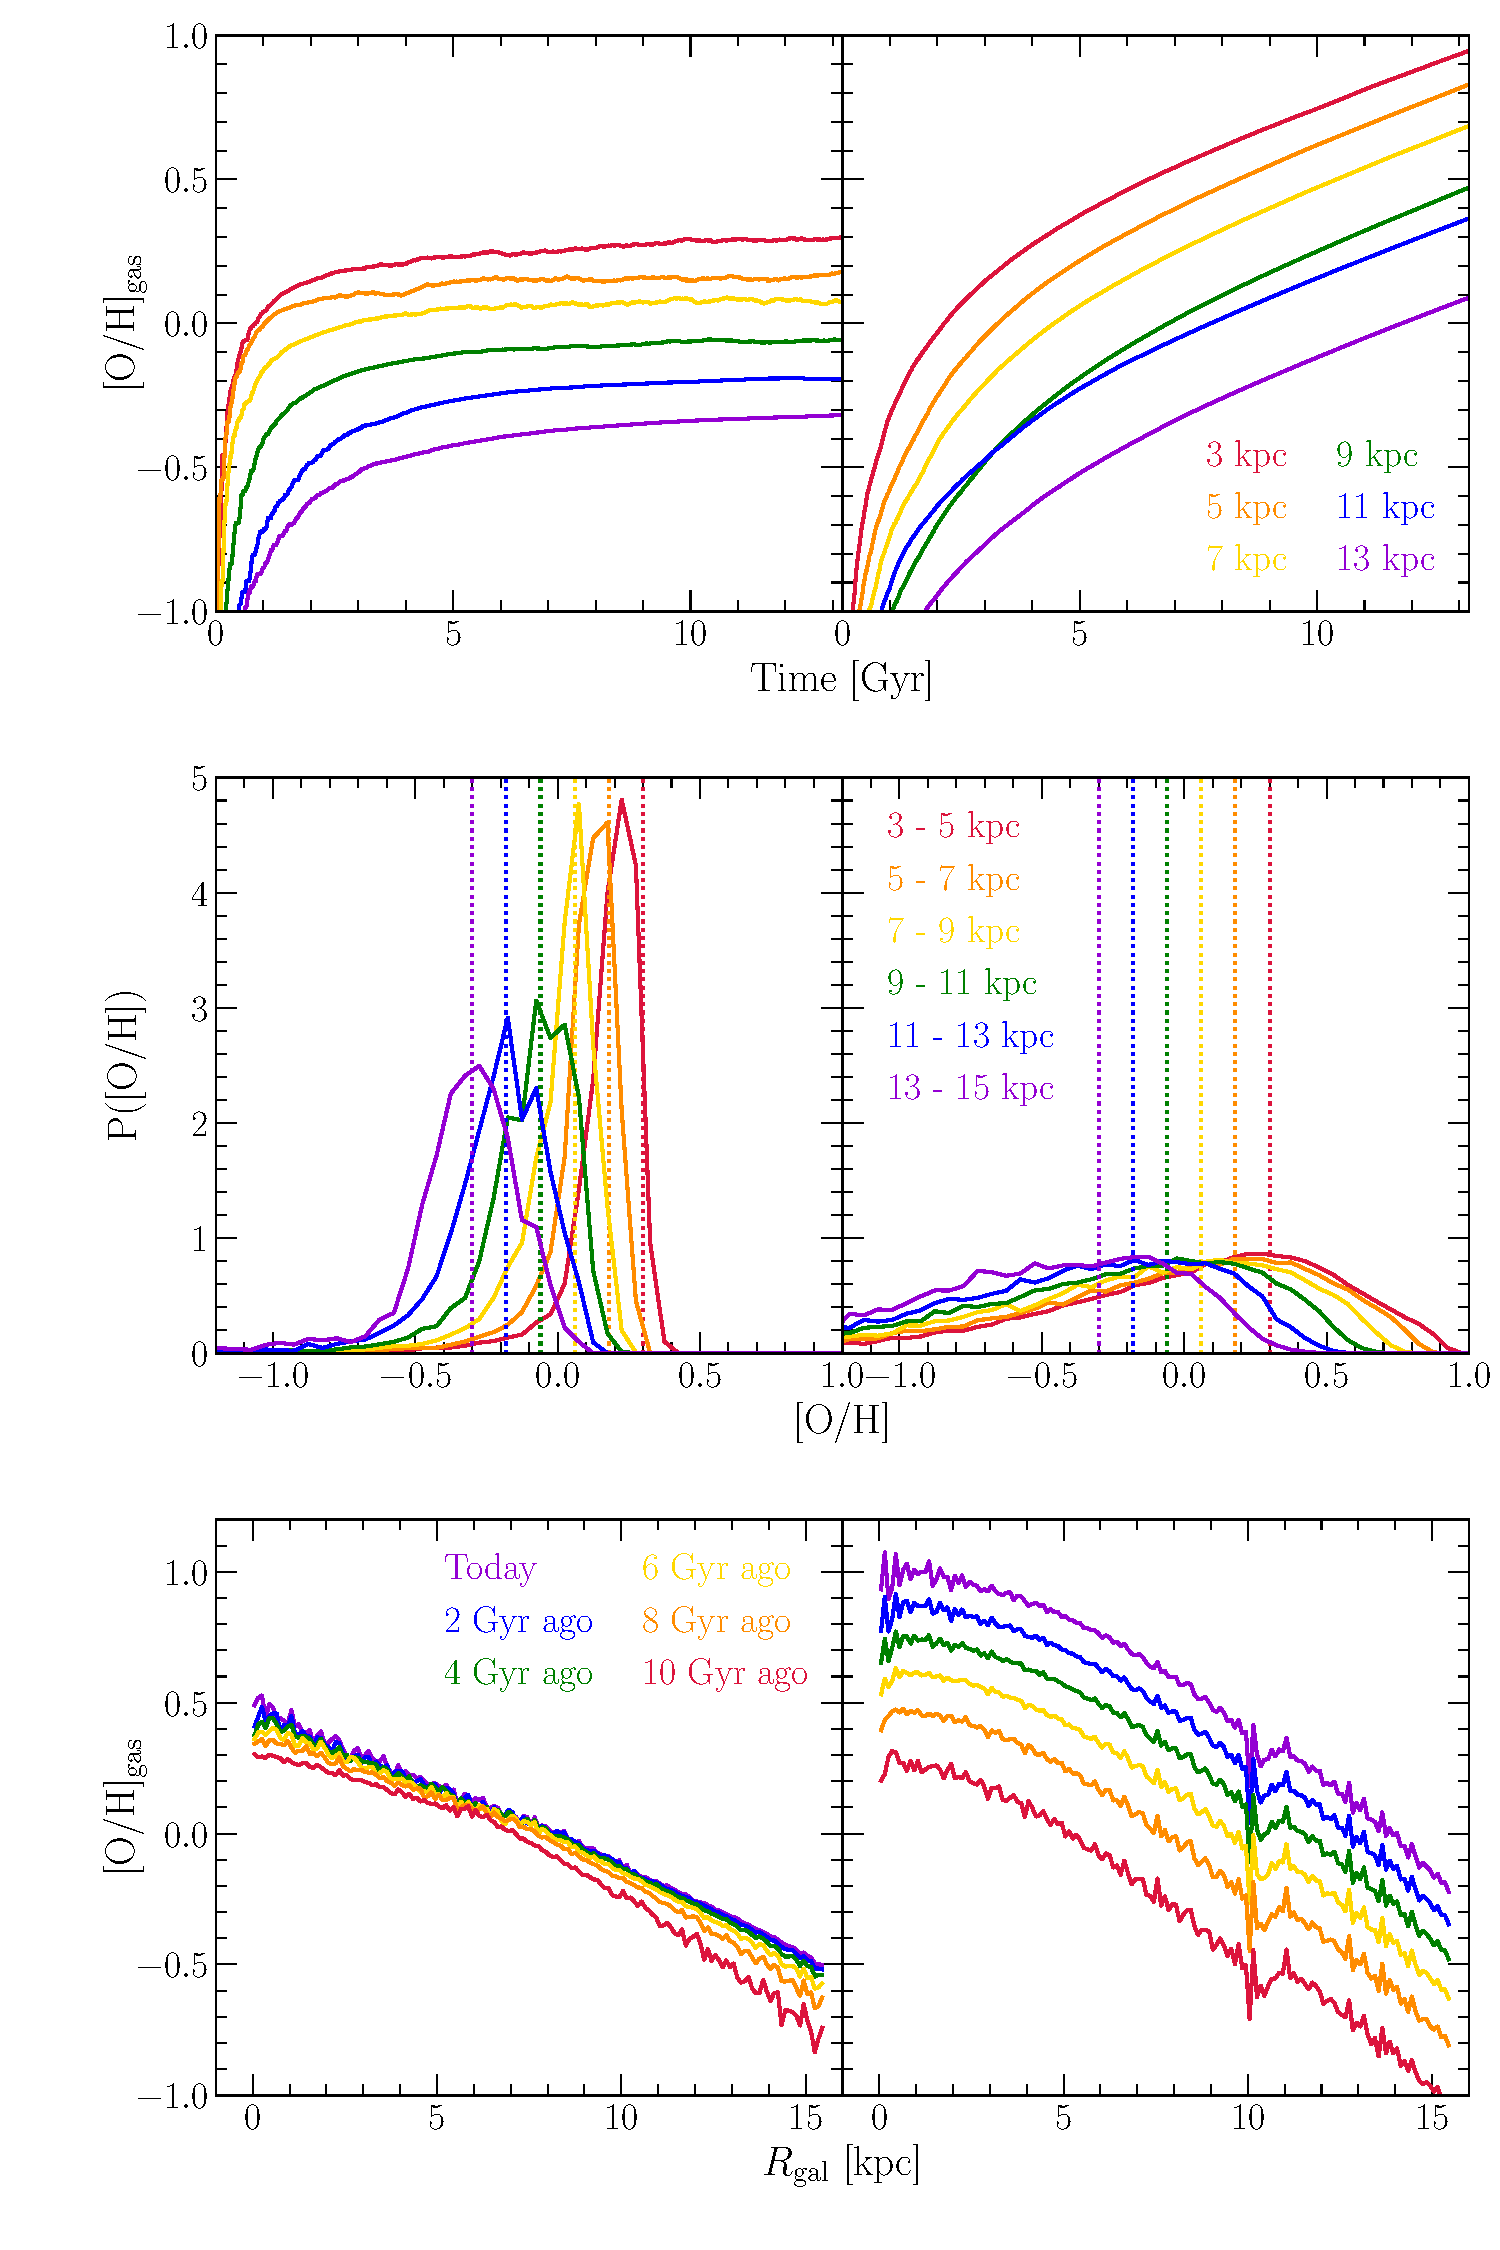
\includegraphics[scale = 0.5]{simplified-examples.pdf}
% \caption{
% Predicted evolutionary histories of the~$\eta \propto e^R$ (left) and
% $\eta = 0$ (right) simplified examples:~\oh~in the ISM at a selection of radii
% (top), the distributions in [O/H] in radial bins (middle), and radial
% gradients in the gas-phase at snapshots between 2-Gyr intervals (bottom).
% Each pair of panels has its own legend identifying the individual curves.
% Vertical dotted lines mark the position of the ``target'' gradient with a
% slope of~$\grad{O} = -0.06$ kpc$^{-1}$ as measured from our APOGEE sample
% in~\S~\ref{outflows:sec:empirical:gradients}.
% }
% \label{outflows:fig:simplified-examples}
% \end{figure*}

% Fig.~\ref{outflows:fig:simplified-examples-sfhs} shows the SFHs of these
% example models.
% The e-folding timescale~\timescale{sfh} varies only marginally with radius
% ($3 - 5$ Gyr across most radii), indicating that it is mostly the increase
% in~$\tau_\star$ driving the abundance gradient.
% Fig.~\ref{outflows:fig:simplified-examples} shows the predicted enrichment
% histories.
% The build up of metals in the ISM is fundamentally different between these two
% models.
% In the case of~$\eta \propto e^R$,~\oh~increases quickly at early times at all
% radii, but reaches the equilibrium abundance after~$\sim$$2 - 3$ Gyr in the
% inner disk and~$\sim$$4 - 5$ Gyr in the outer disk.
% With~$\eta = 0$, abundances increase up to the present day.
% There is an equilibrium abundance in this model, but it is significantly
% super-solar, and it simply takes much longer than a Hubble time to reach it.
% \par
% The differences in metal build up leave a distinct imprint on the stellar
% abundance distributions.
% In the equilibrium scenario, the distributions are strongly peaked, whereas
% they are much broader without mass loading.
% In the former, this prediction arises because the ISM forms stars at a similar
% abundance for most of the disk lifetime.
% In the latter, the peak of the MDF occurs at the ``sweet spot'' calibrated
% above, when the rate of star formation becomes too low to populate the upper
% end of the MDF.
% Due to the ongoing build up of metals without mass loading, the MDF is much
% broader.
% The ISM simply spends much less time forming stars at one distinct abundance.
% \par
% The continual build up of metals also leaves distinct features in the gas-phase
% gradient at different snapshots in time.
% The signature left behind on the radial gradient is an increase in the overall
% normalization over time, while the shape remains largely constant.
% The equilibrium scenario, by its very nature, instead produces a gradient that
% evolves very little between redshift~$z \approx 2$ and the present day.
% \par
% Lastly, we note an additional reason for choosing the mode as our summary
% statistic in quantifying stellar abundance gradients.
% The middle row of Fig.~\ref{outflows:fig:simplified-examples} marks the
% expected value of~\oh~from our linear fit to the gradient
% in~\S~\ref{outflows:sec:empirical:gradients}.
% In both models, the MDF peaks extremely close to its intended position.
% The only noticeable exception is the~$R = 3 - 5$ kpc bin in the
% $\eta \propto e^R$ model, though the difference is~$< 0.1$ dex anyway.
% The match between the intended and actual position of the mode is less
% obvious in the~$\eta = 0$ model due to the broad nature of the MDFs, so we have
% zoomed in on these distributions to verify that they do indeed match well.
% At any given radius, stellar migration enhances the metal-rich and metal-poor
% tails of the MDF with stars from small~$R$ and large~$R$, respectively.
% However, the mode is largely unaffected, indicating that its information
% content on the enrichment history in a given Galactic region is relatively
% uncontaminated by migration.
% The median and especially the mean, on the other hand, are sensitive to the
% tails of the MDF.

% \subsection{Calibrating to the Gas-Phase Gradient}
% \label{outflows:sec:calibrated-model}

% We now calibrate a model with~$\eta = 0$ to reproduce the gas-phase gradient at
% the present day.
% While this observable arises as a consequence of the~$\eta \propto e^R$
% specification in Chapter~\ref{migration}, it depends much more strongly on the
% detailed SFH without mass loading.
% To this end, we take the inside-out SFH (see
% equation~\ref{outflows:eq:inside-out-sfh}) and tune~\timescale{rise}
% and~\timescale{sfh} such that the present-day ISM abundances line up with
% \citeauthor{MendezDelgado2022}'s~\citeyearpar{MendezDelgado2022} measurements
% (see Fig.~\ref{outflows:fig:gradxh-gradage} and discussion
% in~\S~\ref{outflows:sec:empirical:gradients}).
% \par
% Drawing on the results of~\S~\ref{outflows:sec:gce:onezone:simple-cases}, the
% build up of O in the ISM will proceed according to the appropriate form
% of~$f_\text{sfh}$ from Table~\ref{outflows:fig:f-sfh-forms}, modulo the impact
% of stellar migration and radial flows.
% As a fiducial choice of parameters, we retain~$R_g = 3$ kpc,
% $\tau_{\star,0} = 2$ Gyr,~$\eta = 0$,~$\grad{O} = -0.06$ kpc$^{-1}$,~$N = 1.5$,
% and~$v_g = 0$ from~\S~\ref{outflows:sec:simplified-example} above.
% Given these choices, the only remaining unknowns before the full time evolution
% of~$Z_\text{O}(t)$ is known are~\timescale{rise} and~\timescale{sfh}.

% \begin{landscape}
% \begin{figure*}
% \centering
% 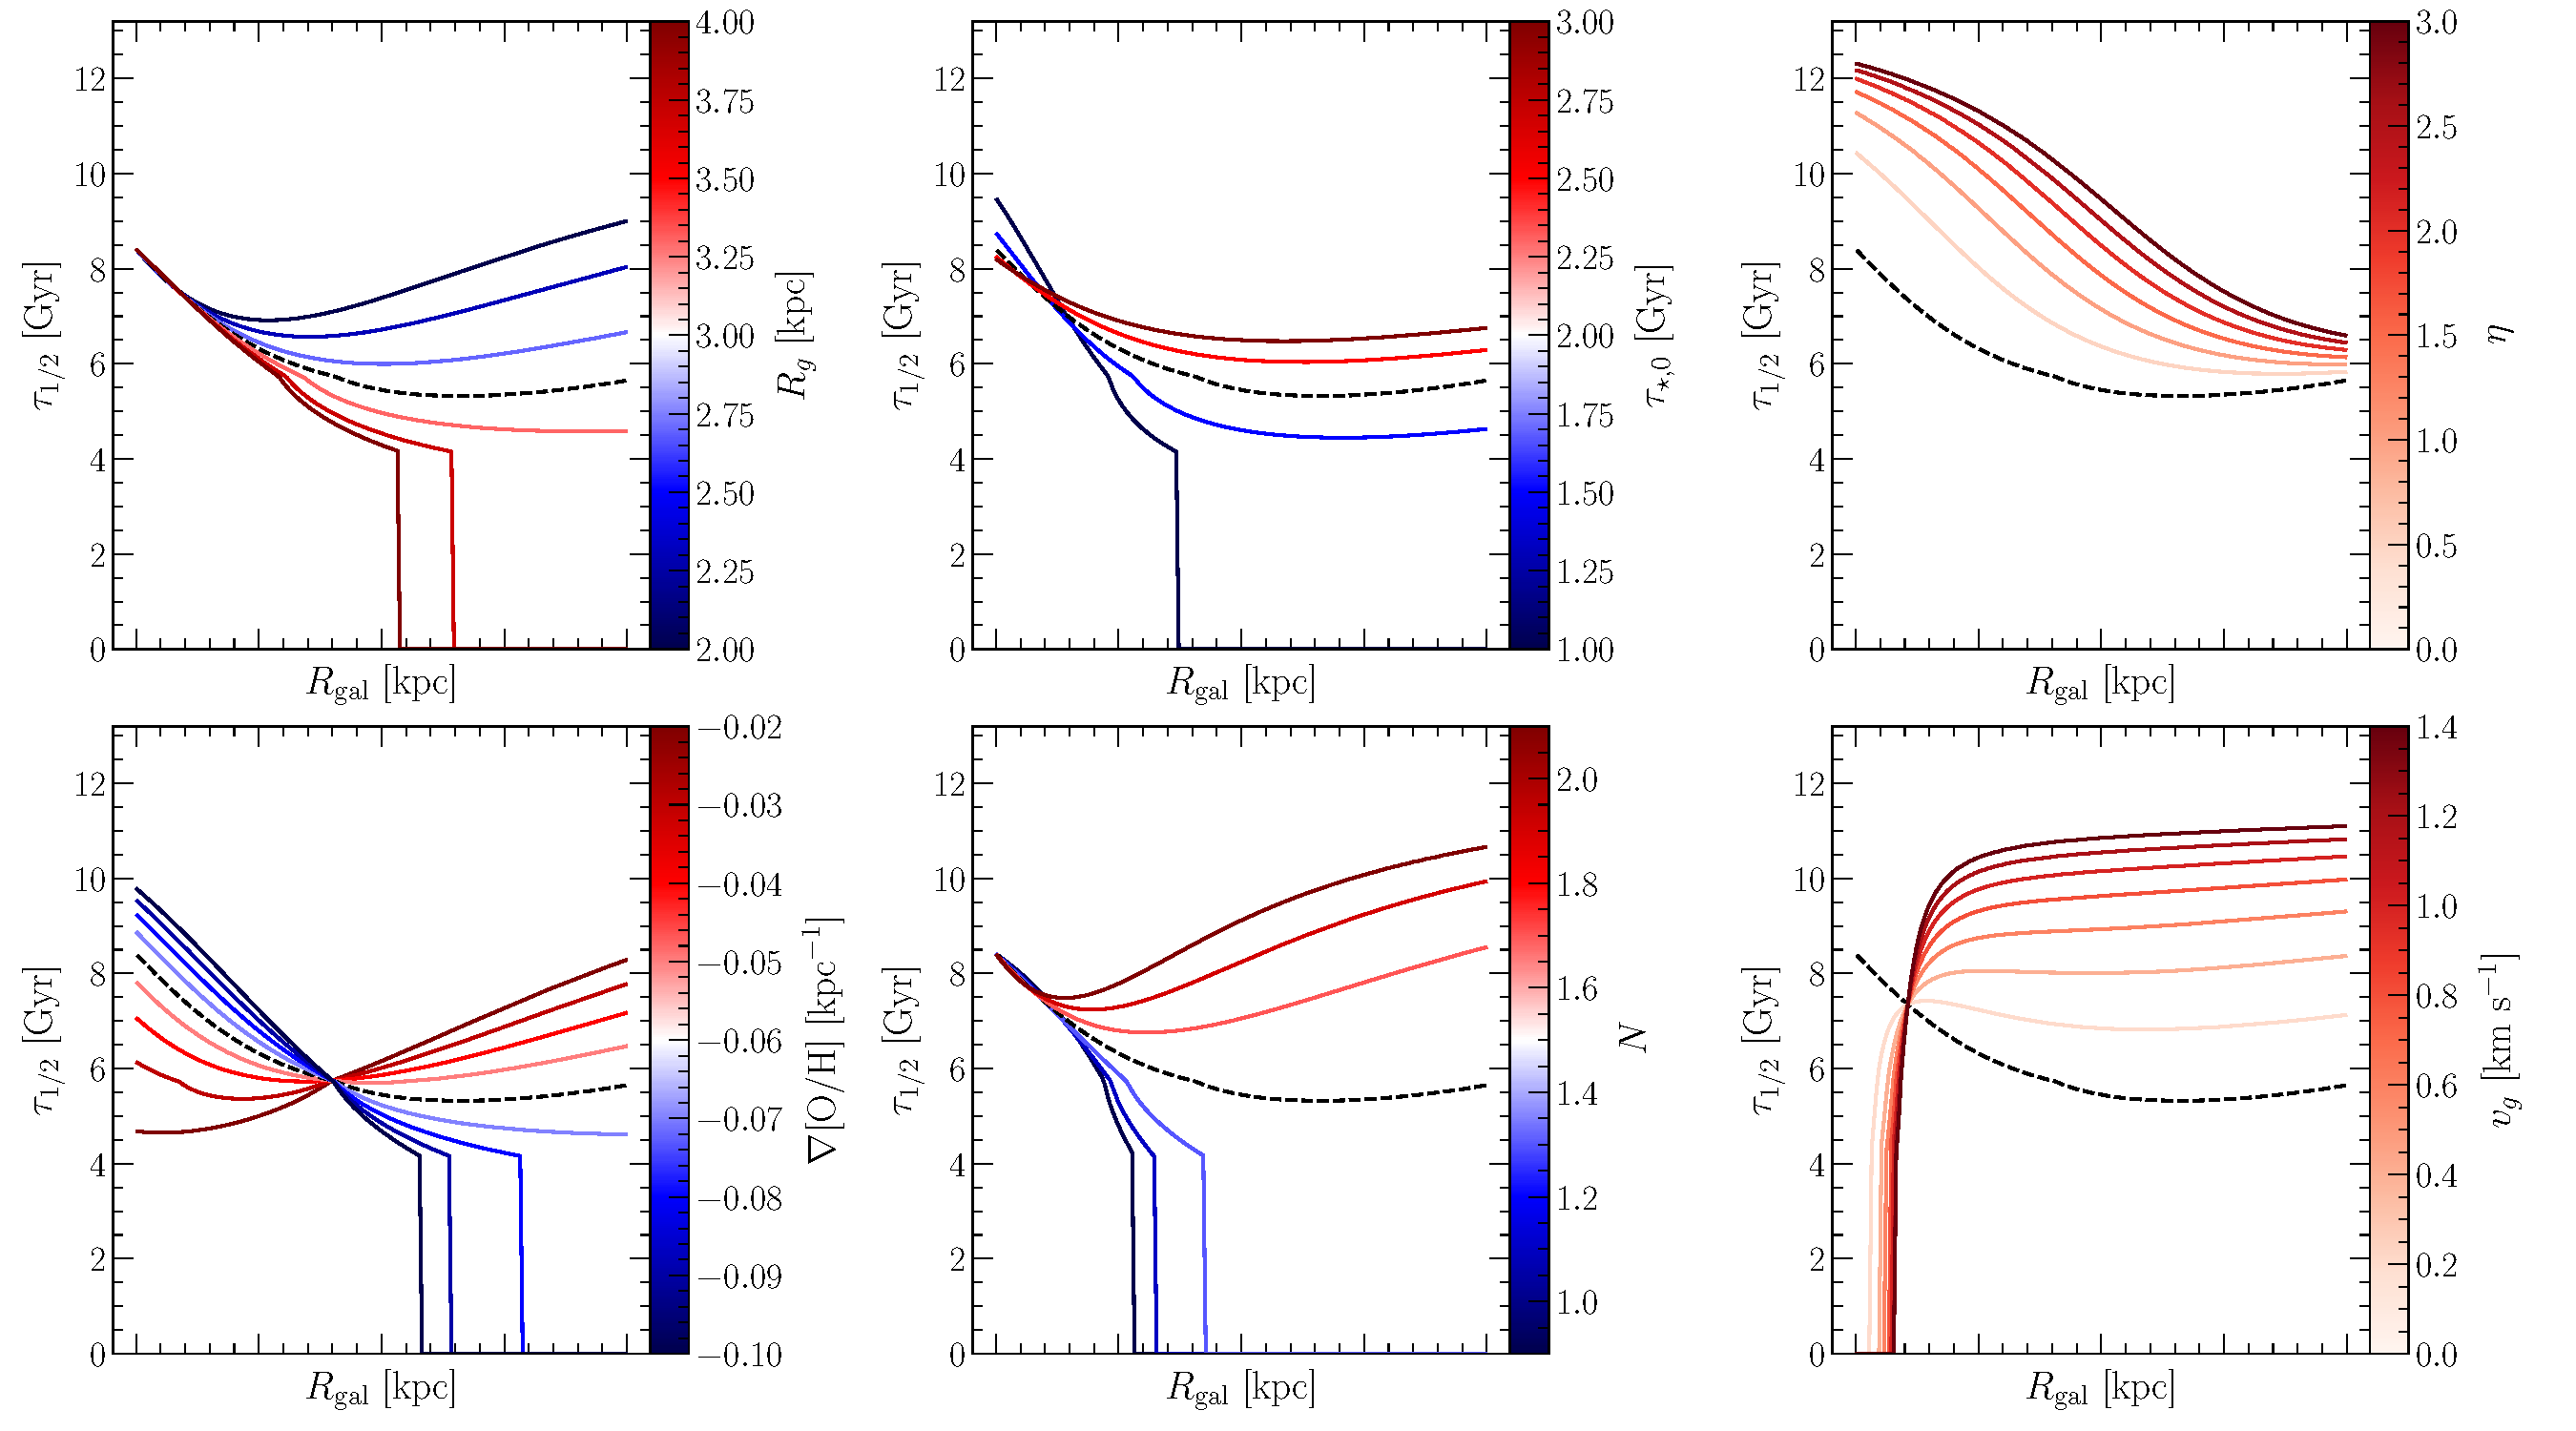
\includegraphics[scale = 0.4]{medage_inputparams.pdf}
% \caption{
% Median age as a function of radius.
% }
% \label{outflows:fig:medage-inputparams}
% \end{figure*}
% \end{landscape}

% Following Chapter~\ref{migration}, we initially set the rise timescale
% to~$\timescale{rise} = 2$ Gyr.
% We then attempt to solve for~\timescale{sfh} via bisection.
% If the value exceeds~$\timescale{sfh} = 200$ Gyr (essentially flat
% at~$t >> \timescale{rise}$), we then hold it fixed there and solve for the
% value of~\timescale{rise}.
% If this value also exceeds~$200$ Gyr, then we conclude that there is no
% physical solution under the given parameter choice.
% We then map~\timescale{rise} and~\timescale{sfh} to the median age of stellar
% populations~$\tau_{1/2}$ by integrating over the implied SFH with an assumed
% disk lifetime of~$\timescale{disk} = 13.2$ Gyr.
% \par
% {\color{red} Potentially move this to a discussion section.}
% Fig.~\ref{outflows:fig:medage-inputparams} shows the results of applying this
% procedure as a function of radius and exploring variations in the individual
% parameters.
% The sensitivity of the predicted age gradient to the input parameters
% underscores a key difference between the~$\eta = 0$ and~$\eta \propto e^R$
% scenarios.
% Without mass loading and variations thereof with radius, the shape of the SFH
% is all there is to vary between Galactic regions.
% If the shape of the SFH (i.e., inside-out galaxy growth) is the primary
% mechanism behind the radial abundance gradient, then it is directly connected
% to the age gradient.
% \par

